\chapter{Discovering the Temporal Perspective}

\todo[inline]{BPM1. Organize the chapter.}

%The class of processes that we discuss in this chapter are long-term engineering
%projects. These processes have specific requirements for monitoring. First, they
%are executed only once according to the specific needs of a particular project, and
%only partially according to recurring process descriptions. Second, they involve
%various actors that typically document their work in a semi-structured way using
%text and tables. Third, work in the project is usually subject to constraints
%regarding the start and end and the temporal order. Fourth, there is typically
%no process engine controlling the execution. Fifth, even though these limitations
%in terms of traceability exist, there are usually strong requirements in terms of
%tracking when which work was conducted.
%
%
%Here goes the contribution from BPM1. 

%\section{Introduction}
This chapter introduces artifact A1. It develops concepts to capture software development as a specific types of process, namely project-oriented. 
The rest of this chapter is structured as follows. Section~\ref{sec:bpm2015background} describes the research problem and summarizes insights from prior research upon which our project mining approach is built. \Cref{sec:bpm2015related} describes the related work. Section~\ref{sec:bpm2015concept} defines the preliminaries of our work and presents an algorithm to mine project-oriented business processes. Section~\ref{sec:bpm2015evaluation} describes the implementation of this algorithm and discusses the results from its application to VCS logs from a real-world engineering project. Section~\ref{sec:bpm2015discuss} highlights the implications of this work before Section~\ref{sec:bpm2015outro} concludes. 




make a cover page: see Jan's picture in Skype chat

In this there is the abstract and there are informations about what research question it addresses, where it was submitted




\section{The Problem of Time Perspective Discovery} \label{sec:bpm2015background}
%\section{Background}
\label{sec:bpm2015background}

Business process management plays an important role for improving the performance and compliance of various types of processes. In practice, many processes are executed with clear guidelines and regulatory rules, but without an explicit centralized control imposed by a process engine. In particular, it is often important to exactly know when which work was done. This is, for instance, the case for complex engineering processes in which different parties are involved. We refer to this class of processes as project-oriented business processes.

Such project-oriented business processes are difficult to control due to the lack of a centralized process engine. However, there are various unstructured pieces of information available to analyze and monitor their progress. One type of data that are often available these processes is event data from version control systems (VCS). While process mining techniques provide a useful perspective on how such event data can be analyzed, they do not produce output that is readily organized according to the project orientation of these processes.

In this thesis, we define formal concepts for capturing project-oriented processes. These concepts provide the foundation for us to develop an automatic discovery technique which we refer to as \emph{project mining}. The output of our project mining algorithm is organized according to the specific structure typically encountered in project-oriented business processes. With this work, we extend the field of process mining towards the coverage of this specific type of business process.


Next, we describe the addressed problem and related work.


\subsection{Problem Description}\label{sec:bpm2015problem}
The class of processes that we discuss in this paper are long-term engineering projects. These processes have specific requirements for monitoring. First, they are executed only once according to the specific needs of a particular project, and only partially according to recurring process descriptions. Second, they involve various actors that typically document their work in a semi-structured way using text and tables. Third, work in the project is usually subject to constraints regarding the start and end and the temporal order. Fourth, there is typically no process engine controlling the execution. Fifth, even though these limitations in terms of traceability exist, there are usually strong requirements in terms of tracking when which work was conducted.

%Unlike other types of business processes, the processes we consider here
%representing such projects are specifically tailored to customer needs the specific needs of the project, and there is

In line with these observations, a \textit{project-oriented business process} can be defined as an ad-hoc plan that specifies the tasks to be performed within a limited period of time and with a limited set of resources for achieving a specific goal. Unlike repetitive business processes for which notations such as BPMN~\citep{bpmn2_stable} or EPC~\citep{vanderaalst_formalization_1999} are commonly used, project-oriented business processes may be properly represented with PERT or GANTT models. The concept is illustrated in Fig.~\ref{fig:bpm2015problem}.


\begin{figure}[tb]
\centering
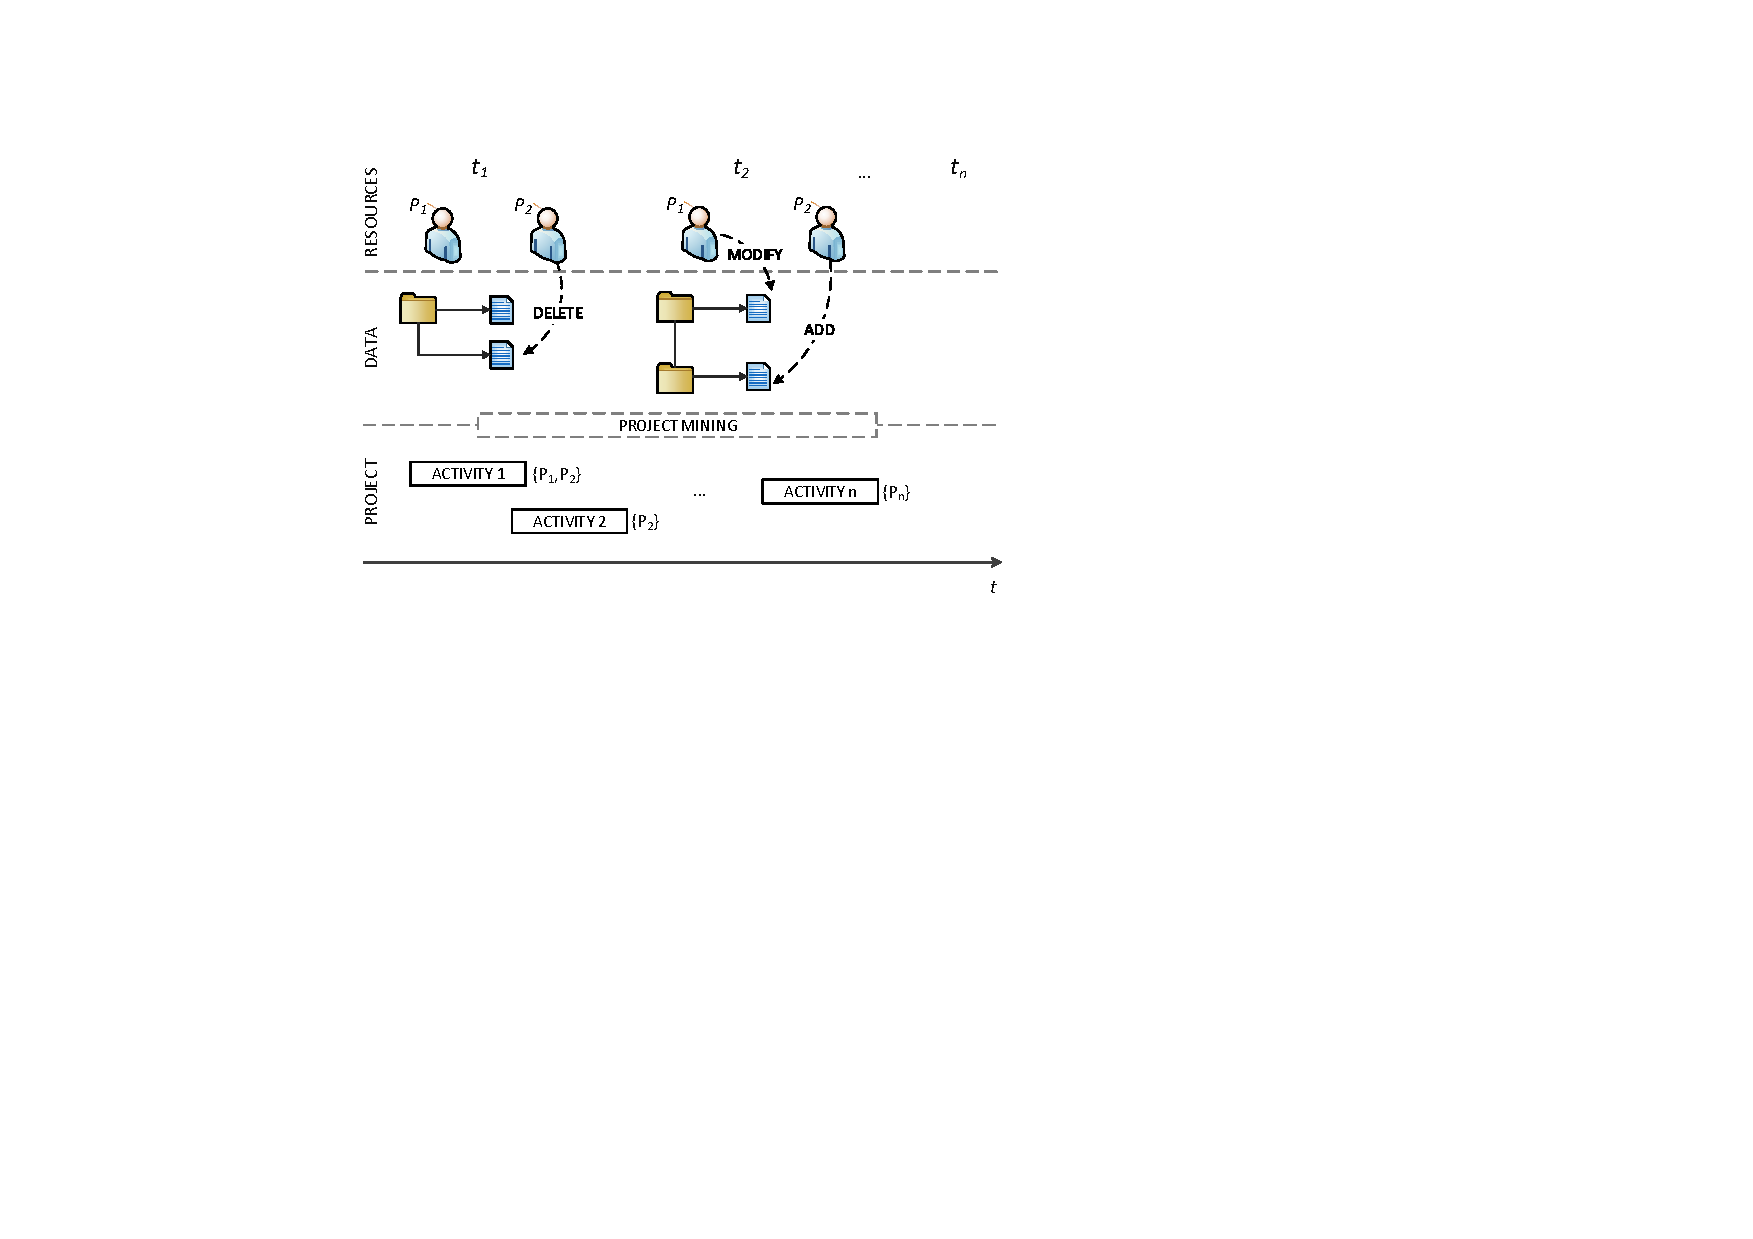
\includegraphics[width=.8\textwidth]{bpm2015/imgs/ProjectMining.pdf}
\caption{Problem illustration}
\label{fig:bpm2015problem}
\end{figure}

Documentation is required not only explicitly as part of some activities but also to comply with norms and regulations that may require some evidence of the actions being performed in the organization. Documents are usually free of format or contain tables, at best. The unstructuredness of data makes it difficult to monitor processes and check rules on them. A starting point for analysis of project-oriented processes can be data logs %generated for  %usually consist of subversion projects
that are stored in Software Configuration Management (SCM) systems that help tracking the evolution of data and restore information if needed~\citep{voinea_open_2006}.
However, hundreds of versions of thousands of files are common in a single project~\citep{voinea_multiscale_2006}, which makes it impractical to browse this data manually.

%We focus on project mining motivated by a real case scenario in the scope of the SHAPE research project\footnote{\url{http://ai.wu.ac.at/shape-project/}}.
%The data log is provided by a Version Control Systems (VCS) whose information is not subdivided into traces related to process instances but consists of a hierarchy of work streams associated with individual files being added, modified or deleted in a subversion repository.

Let us see an example inspired by a real scenario of a process to write a project proposal that uses a Version Control System (VCS) to store the data. The project history, and hence, the data produced, starts when people begin to work on the proposal, which involves a description of the project goals and milestones, a division of tasks into work packages, an estimation of cost and resources required, etcetera. This information is spread in the repository over several folders containing different documents, which are later merged into a single file. If the proposal is accepted, the first step is to organize a kickoff meeting and assign specific resources to the work packages. A hierarchical set of folders is then created in the repository in order to store the information generated for each work package. As the project evolves over time, resources contribute by adding, removing or modifying information to the VCS repository. %\todo{Should answer point 3 on the review-list: Missing concrete examples of the need to “prove compliance to rules and regulations”. Which important rules and regulations will the analysis help comply with?} 
Project evolution is guided by specific norms that impose the execution of predefined steps. For instance, the European norm EN5016 requires a preliminary \gls{ram} analysis to support targets. 
%Data stored in the VCS can be used to prove compliance to rules and regulations of the domain. For instance, in the railway industry, 

Table~\ref{tab:bpm2015example} depicts an excerpt of the log data generated, where the first column (on the left hand side) indicates the commit identifier, the second column indicates the person who committed changes, the third column indicates the commit date, %the fourth column shows (optional) descriptive information to clarify the scope of the changes performed
and the fourth column indicates the files affected and the type of action performed among added (A), modified (M) and deleted (D).
For the sake of simplicity, the table shows the log data of a specific time period and the actions related to a specific task, namely, $\defineExample$. That task was assigned to resource X % after a project meeting. %, when a part of project members asked for a toy example to better understand the problem domain.
and was supervised by resource Y and, later on, also by resource Z.
%An extract from the log concerning this period, that shows some crucial steps in the \emph{example} task, is reported on table \ref{tab:example}. Comments were left out from this representation, since at the current state we don't delve into them.

\begin{table}[bt]
\caption{Excerpt from VCS log data for the referenced time period }
\label{tab:bpm2015example}
%\scriptsize
{
%	\renewcommand{\arraystretch}{1.3}
\centering
%\fontfamily{phv}\fontseries{mc}\selectfont
\begin{tabular}{m{.8cm} m{1.5cm} m{3cm} p{5.8cm}}
%\hline\noalign{\smallskip}
%\hline
\toprule
\textbf{CID}	 & \textbf{Resource} & \textbf{Date} & \textbf{List of changes} \\
%\noalign{\smallskip}
%\hline
%\noalign{\smallskip}
%\hline
\midrule
%\noalign{\smallskip}
\multirow{2}{*}{1} & \multirow{2}{*}{Y} & \multirow{2}{*}{2014-11-12~11:57:46} & A /example \\
& & & A \slash example\slash SHAPE\slash\-ToyStation\-Example.docx \\ \midrule %\hdashline

%\multirow{2}{*}{205} & \multirow{2}{*}{X} & \multirow{2}{*}{2014-11-14 16:26:23} & A /example/ToyStation.bpmn \\
%& & & A /example/ToyStation.png \\ \hline %\hdashline

\ldots & \ldots & \ldots & \ldots \\ \midrule

%\noalign{\smallskip}
\multirow{2}{*}{3} & \multirow{2}{*}{X} & \multirow{2}{*}{2014-11-14 16:34:07} & M /example/ToyStation.bpmn\\
& & & M /example/ToyStation.png \\ \midrule%\hdashline

%\multirow{7}{*}{207} & \multirow{7}{*}{X} & \multirow{7}{*}{2014-11-27 14:18:59} & M /example/SHAPE-ToyStation-Example.docx \\
%& & & D /example/ToyStation.bpmn \\
%& & & M /example/ToyStation.png \\
%& & & A /example/ToyStation\_0Loop.bpmn \\
%& & & A /example/ToyStation\_1Loop.bpmn \\
%& & & A /example/ToyStation\_nLoop.bpmn \\
%& & & A/example/ToyStation\_old.bpmn\\ \hline

%\ldots & \ldots & \ldots & \ldots \\ \hline

%\noalign{\smallskip}
4 & W & 2014-12-15 13:49:11 & D /example/Download \\ \midrule %\hdashline

%\noalign{\smallskip}
5 & W & 2015-01-08 16:06:41 & A /example/Download2\\ \midrule %\hdashline

%\noalign{\smallskip}
\multirow{2}{*}{6} & \multirow{2}{*}{X} & \multirow{2}{*}{2015-01-13 11:47:09} & M /example/ToyStation\_0Loop.bpmn\\
& & & M /example/ToyStation\_nLoop.bpmn \\ \midrule %\hdashline

%\noalign{\smallskip}
\multirow{2}{*}{7} & \multirow{2}{*}{Z} & \multirow{2}{*}{2015-01-16 16:50:29} & A /example/ToyStation\_0Loop.pdf\\
& & & A /example/ToyStation-feedbackZ.pdf\\ \bottomrule %\hdashline
\end{tabular}\\ 
}
\end{table}

%Process mining techniques can help to discover processes from log data.
%Existing process mining techniques can deal very well with execution logs whose data is subdivided into \textit{traces} representing different process instances in which events are easily identifiable (e.g. through a \textit{caseId}).
%Procedural (e.g. BPMN~\citep{bpmn2_stable}, Petri nets~\citep{aalst_application_1998}, EPC~\citep{vanderaalst_formalization_1999}) as well as declarative (e.g. Declare~\citep{VanderAalst2009}, DPIL~\citep{zeising2014towards}) modeling languages can be used to represent the process discovered.
%Once a process model is discovered, it can be checked whether it is compliant with the existing (already known) process model and enhance the model or the way the process is executed accordingly.
%Performance can also be analyzed and compared to the expected values defined by key performance indicators (KPIs)~\citep{delrioortega_definition_2013}.

%\begin{table}[bt]
%\caption{Process mining vs. project mining}\label{tab:processVSprojectmining}
%\centering
%\begin{tabular}{l c c}
%%\hline\noalign{\smallskip}
%%\hline
% ~&~  Process Mining~&~Project Mining\\
%%\noalign{\smallskip}
%\hline
%%\noalign{\smallskip}
%Defined goals~&~  \cmark ~&~ \cmark \\
%Resource~&~ \cmark ~&~ \cmark \\
%Activities/Tasks~&~ \cmark ~&~ \cmark \\
%One time~&~ \xmark ~&~ \cmark \\
%Repetitive~&~ \cmark ~&~ \xmark \\
%\hline \\
%\end{tabular}
%\end{table}

%However, due to the ad-hoc nature of project-oriented business processes, the event logs for these processes look different.
%Therefore, mining of project-oriented business processes needs to be done in a different way.
%Whereas in traditional process mining the main goal is to discover the execution order and relation among activities, project mining aims at discovering the structure of the project along with its temporal progress and information about the actors involved.

% Deviations from the designed plan can then be measured, as well as the fulfillment of milestones, deadlines, resource usage constraints, cost expense, etcetera. Table~\ref{tab:processVSprojectmining} illustrates the main differences between process mining and project mining concepts\todo{CC: I'm not sure whether this table is representative and/or necessary}.


%\begin{table}[bt]
%\centering \begin{tabular}{m{1cm} m{2cm} m{2.8cm} m{3cm} l}
%%\hline\noalign{\smallskip
%\hline
%CID	&	Resource	&	Date	&	Message	&	List of changes \\
%%\noalign{\smallskip}
%\hline
%%\noalign{\smallskip}
%\hline
%\multirow{3}{*}{1} & \multirow{3}{*}{pol@uni.edu} & \multirow{3}{*}{2006-02-17 15:30} & \multirow{3}{*}{} & A /templates \\
%& & & & A /temp/costsplan.doc \\
%& & & & A /temp/proposal.pdf \\ \hline %\hdashline
%\multirow{3}{*}{2} & \multirow{3}{*}{al@co.com} & \multirow{3}{*}{2006-02-19 12:00} & \multirow{3}{*}{Reviewed proposal} & A /slides \\
%& & & & A /slides/review.doc \\
%& & & & M /temp/proposal.pdf \\ \hline %\hdashline
%\multirow{2}{*}{3} & \multirow{2}{*}{al@co.com} & \multirow{2}{*}{2006-02-19 17:05} & \multirow{2}{*}{Renamed a file} & D /temp/proposal.pdf \\
%& & & & A /temp/proposal\_final.pdf \\ \hline %\hdashline
%\multirow{2}{*}{4} & \multirow{2}{*}{jb@uni.edu} & \multirow{2}{*}{2006-02-23 11:05} & \multirow{2}{*}{Added CV} & \multirow{2}{*}{A /skills/CV.pdf} \\
%& & & & \\ \hline %\hdashline
%\multirow{2}{*}{5} & \multirow{2}{*}{ccm@uni.edu} & \multirow{2}{*}{2006-02-19 17:05} & \multirow{2}{*}{WPs description} & A /goals/WPS\_description.doc \\
%& & & & M /temp/costsplan.doc \\ \hline %\hdashline
%\multirow{2}{*}{\ldots} & \multirow{2}{*}{\ldots} & \multirow{2}{*}{\ldots} & \multirow{2}{*}{\ldots} & \multirow{2}{*}{\ldots} \\
%& & & & \\ \hline
%\end{tabular}\\ \hfill
%\caption{A representation of VCS log data}
%\label{tab:VCSlog}
%\end{table}

%\begin{figure}
%\centering
%\includegraphics[height=6.2cm]{imgs/pm-pic}
%\caption{Problem illustration,}
%\label{fig:example}
%\end{figure}

Existing frameworks, such as Subversion or Git, allow to access their logs in different ways. However, the covered information is limited to (roughly) that depicted in Table~\ref{tab:bpm2015example}. Especially for big projects that are frequently updated over a large period of time, these logs are complex to analyze.
Therefore, the problem to address is how to analyze and visualize the information produced in project-oriented business processes such that it can be represented in an understandable and manageable way by project experts and
enable, a.o., the automation of mechanisms for compliance checking.
The following properties of project-oriented process logs must be taken into account to achieve this goal: (i) VCS repositories consist of a hierarchy of folders and files which are logically organized such that work is grouped in a specific way; (ii) process activities are not registered in VCS log entries. Therefore, such information must be inferred by reasoning on the repository structure and/or the content of the log entries; (iii) the granularity of the events is unknown a priori and it needs to be defined before analyzing the data.
%Therefore, the goal of project mining is to represent that data in a way that is natural to the project (i.e., by deriving the project structure and its progress over time) taking into consideration the aforementioned properties of VCS logs.

%\begin{itemize}
%\item we cannot see activities, but we can see that work was done
%\item hierarchical work structure (requirements)
%\item names of activities are not directly explicit
%\item granularity of events (e.g. in our case is on the file level)
%\end{itemize}

%We need to retrospect that the things that we did in the project were complete and correct. Answer to questions like: Did we do all the stuff?\\ \hfill

%Logs carry much more information (such as the number of lines or bytes modified in a file) but for the moment let's treat only this level of granularity.

%\todo[inline]{CC: Some further work is required on sections 2.1 and 2.2 so that the transition from the former to the latter is smooth and the last part of section 2.2 makes sense}


\subsection{Related Work}
\label{sec:bpm2015related}

The problem described has been addressed in the literature from different perspectives. The first category of related work tackles the problem by transforming it into a process mining problem. Consequently, approaches have been developed to preprocess VCS data such that process mining techniques can be applied, and hence, a business process can be derived from the log data.
In this group, Kindler et al. \citep{Kindler2006,kindler2006incremental} developed an algorithm for extracting software processes that are mapped to Petri Nets. Activities, which are not explicit in the logs, are discovered from their input and output artifacts. However, strong assumptions are made on the filenames as well as on the software process lifecycle. %(always design, code, review, testres). Activities (which are not explicit in the logs, like in our case) are discovered from their input and output artifacts. Here defined as triples $<I,O,R>$ where I=input, O=Output, R=resouce who perfomed it.
Rubin et al. in \citep{rubin2007process} addressed the problem of engineering processes that are not well documented and are usually unstructured. They provided a bridge from Kindler et al.'s approach to ProM \citep{van2005prom} in order to mine different process perspectives, such as performance social network analyses. %but not from a project point of view.
Rubin et al. \citep{rubin2014agile} applied process mining to the touristic industry and obtained user processes from web client logs pursuing the goal of improving the software system by analyzing the underlying process.
Poncin et al. \citep{Poncin2011a} developed the FRASR framework for preprocessing software repositories to transform the VCS data to logs that conform to the process mining event log meta model~\citep{van2005meta} as utilized in ProM \citep{van2005prom}.
However, these approaches disregard the single-instance nature of project-oriented business processes and treat them as procedures that can be repeated over time.

The second category of related work focuses on the visualization of VCS data %by defining measurements such as things that can be plotted into a chart.
for different purposes.
%There are two main lines of how this problem was approached in literature.
%\paragraph*{visualization perspective} defining measurements such as things that can be plotted into a chart. But, they haven't any explicit notion of work structure.
%\paragraph*{preprocessing} - VCS data is transformed in order to comply to the process mining meta model from van Dongen and van der Aalst \citep{van2005meta}. This means that they are oriented to discover "classical" processing (i.e. repeated many times in the logs).
Several approaches study the interaction among developers over time from a visualization point of view. For instance, Ogawa and Ma \citep{ogawa2010software} drew storyline pathways to show the story of each developer's contribution. Other approaches analyze and visualize VCS data at file level in order to discover file version evolution. Voinea and Telea~\citep{voinea_multiscale_2006} introduced an interactive navigation method to surf file version evolution as well as two methods to cluster versions of the same file in an abstraction layer. Wu et al.~\citep{jingwei_evolution_2004} also visualized the evolutions of entire projects at file level, emphasizing the evolution moments.
Finally, several approaches study change prediction with the aim of discovering prediction patterns that can help in the process of software development~\citep{zimmermann_mining_2004,ying_predicting_2004}.
%Feld et al. \citep{feldt2013supporting} used software project data to \emph{predict} potential problems during development. Heatmaps, used to visualize source code changes in a two dimensional space, showed to be easily readable also by non experts.
The approaches mentioned in this category as well as others that apply similar techniques~\citep{feldt2013supporting,kagdi_mining_2006,dambros_flexible_2008} focus on studying software evolution from different standpoints. However, the goal pursued differs in all cases from our goal in that they are not interested in discovering projects tasks out of the log data, and hence, they lack an explicit notion of work structure that we need to consider for our purpose.

Our approach combines ideas from both areas, as we aim at identifying tasks like in the approaches that rely on process mining, but we must cluster the data in an appropriate way, for which techniques developed in the approaches that pursue visualization may be adapted or extended.

%----------------
%
%Then explain that, in our work, we don't only want to see what's happening. We want also compliance (which means: did things happen in the right way (as they were allowed to)? Compliance can be provided by Process Mining algorithms... but we cannot apply process mining techniques directly (because they need logs structured in different ways - not svn/git logs). Thus, we need to adopt this strategy. 

\section{Approach to Discover the Time Perspective}
\todo[inline]{Rephrase here}

%\section{Mining \acs{VCS} Event Data}
\label{sec:bpm2015concept}
In the following, we first formalize the notions encountered in the project mining setting. Then we develop an approach to acquire a hierarchical overview on the project from a repository perspective.

\subsection{Preliminaries}
\glspl{vcs} are used in projects to ensure reliable collaboration. We build our approach on \gls{vcs}. Typically, the workflow in \gls{vcs} is that people work on files (e.g., text, source code, spread sheets) and commit them to the central repository. Project participants comment on their commits so that other participants can better understand the nature of the changes to the files.

Let \Files be the universe of files. Files are organized in a file tree. Therefore, each file $\file \in \Files$ has one parent file. The only file without a parent file is the root file. We capture this information in the parent relation $\parent : \Files \times \Files$. For example, let $\file_p \in \Files$ be the parent of file $\file_c \in \Files$, then $(\file_p, \file_c) \in \parent$.
The transitive closure on the parent files is given by the function $\ancestor : \Files \rightarrow 2^{\Files}$ that returns the set of files along the path to the root.

When project members did a certain amount of work and want to save their current progress, they commit the changes to the \gls{vcs}.
We define changes on files as the events of interest on the lowest granularity.
\begin{definition}[Event] \label{def:bpm2015events}
Let $\Events$ %  = \Files \times \ChangeOperations \times \Timestamps \times \Comments \times \ChangedAmount$
be the set of events. An event $\event \in \Events$ is a four-tuple $(\file, \changeOperation, \timestamp, \comment)$, where
\begin{compactitem}
  \item $\file \in \Files$ is the affected file of the event.
  \item $\changeOperation \in \ChangeOperations =\lbrace\added$, $\modified$, $\deleted \rbrace$ is the change operation on the file with obvious meaning.
  \item $\timestamp \in \Timestamps = \mathbb{N}_0$ represents a unix time stamp marking the time of the event occurrence.
  \item $\comment \in \Sigma^*$ is a comment in natural language text.
%  \item $\changedAmount \in \ChangedAmount$ is the absolute number of changed bytes in comparison to the previous version of the file.
\end{compactitem}
% Let $\ChangeOperations = \lbrace \added$, $\modified$, $\deleted \rbrace$ be the set of change operations on files, \Timestamps represent unix time stamps, and $\Comments \subseteq \Sigma^*$ be comments in natural language text.
% Events $\event \in \Events$ are tuples of the form .
% \todo{TODO: decide, if we need weights on how much of the files changed.
% Also: what about resources?}
%$\file \in \Files$ is a file, $\changeOperation \in \ChangeOperations$ is a change operation, $\timestamp \in \Timestamps$ is a timestamp, and $\comment \subset \Sigma^*$ is a comment in natural language text.
\end{definition}

For events $\event = (\file, \changeOperation, \timestamp, \comment%, \changedAmount
)$ we overload $\file, \changeOperation, \timestamp$, and $\comment$
%,$ and $\changedAmount$ 
to be used as accessor functions. For example, \file is the function $\file : \Events \rightarrow \Files$ mapping an event to its affected file.

Project participants can commit a number of changes to different files at one step. Therefore, we define the notion of commits as follows.
%\todo{Maybe instead use a reduction of an event like $\event_{|\timestamp}$}

\begin{definition}[Commit]
A commit $\commit$ is a set of events sharing the same time stamp and comment, i.e., $\forall \event, \event' \in \commit: \timestamp(\event) = \timestamp(\event') \wedge \comment(\event) = \comment(\event')$. Additionally, each event in a commit affects different files, i.e., $\forall \event, \event' \in \commit : \event \neq \event' \rightarrow \file(\event) \neq \file(\event')$.
\end{definition}
%\todo{Decide: Do we need the definition Commits at all?}

Usually, it is in the hands of project participants, when they decide to commit changes to the \gls{vcs}. In the extreme case, there could be only a single commit made in a project that adds all files to the repository.
Note that this extreme practice would render the use of a \gls{vcs} obsolete. On the contrary, it is common practice to regularly perform commits in order to securely store work progress and to reduce the chance of conflicts~\citep{pilato2008version,Hou2014}. Conflicts occur, when another participant committed changes to a file that is being committed and can cause extra work.
Based on these insights, we make the assumption that commits are regularly made during work.

Projects are decomposed into work packages. We assume a hierarchical work package structure of a project, such that a work package can have sub work packages. Further, the amount of work in a single work package need not be done in one single time span, but it can be split into several activities. Activities have a start and end time, and subsequent activities can have idle periods in between. Thus, we define projects as follows.
\begin{definition}[Project]\label{def:bpm2015project}
A project \Project is a tuple $(\WorkPackages, \Structure, \Activities, \startTimeFunction, \finishTimeFunction, \MappingFunction)$, where
\begin{compactitem}
  \item $\WorkPackages$ is the set of work packages in the project.
  \item $\Structure \subseteq \WorkPackages \times \WorkPackages$ is the relation that hierarchically decomposes work packages into a tree structure.
  \item $\Activities$ is the set of activities that are conducted in the work packages.
  \item $\startTimeFunction : \Activities \rightarrow \Timestamps$ is the function that assigns a start time to activities. Activities are ordered by their start times.
  \item $\finishTimeFunction : \Activities \rightarrow \Timestamps$ is the function that assigns an end time to activities.
  \item $\MappingFunction : \Activities \rightarrow \WorkPackages$ is the mapping function that maps activities to their corresponding work packages.
\end{compactitem}
\end{definition}

Note that this definition reflects an activity centric view on projects. The definition deliberately omits further dimensions, e.g., costs, resources, risks. The idea is not to capture projects in every detail, but to focus on the work packages of a project to obtain an overview of the work that is being done. %\todo{Question: do we want a full-blown definition on projects? with risks, resources, milestones, stakeholders, \ldots?}
We are interested in when work has been started in a work package, and when work packages have been done. This information can be derived from the activities associated to the workpackages. An obvious assumption is that the work package starts with its first activity, and ends when its last activity is completed.

Based on these notions, we can define the task of \emph{project discovery} as reconstructing the project \Project from a set of low level event data \Events.
In the following, we present an approach to this problem.

% \begin{definition}[Project mining]
% 	Given a set of events \Events, the objective of project mining is to identify:
% 	\begin{compactitem}
% 		\item the set of work packages \WorkPackages in the project.
% 		\item the start \startTimeFunction, and end \finishTimeFunction of the workpackages in \WorkPackages.
% 		\item the hierarchical relation \Structure between work packages.
% 		\item the mapping function \MappingFunction that assigns assigns events to a work package.
% 	\end{compactitem}
% \end{definition}


% Inital definition which we have to align to the current \\
% A commit is a set of change operations. $\commit \equiv \lbrace c \in \changeOperation \rbrace \times \comment$ \\
% A change operation is a set of triples $\changeOperation \equiv \lbrace F, W, O \rbrace $ where $F, W, O$ are respectively the file, the weight (how much a change affected the file), and the operation type ($O={modified,added,deleted}$)\\
% Upon the above sets we can define functions such as a modification function (that, for instance, maps the set of files to their weight), or distance(f1, f2) (but for the moment we don't use it).\\ \vfill

% After the last discussion I identified the following concepts to be formalized. So basically we would need to align the initial definition to was follows.
%
% Definitions: \\
% \begin{definition}[Event]
% Event: something that happens at some point in time. Generally in the past. (Primitive concept: can't be derived from any other concepts? Can it be defined?!)
% Event data: data regarding events. An event over a dataset A is the minimum amount of modification made to the minimum part of A at some point in time. i.e. the smallest possible change.
% \end{definition}
%
% \begin{definition}[Project]
% D2. Project (hierarchy) \\
% a project has a hierarchy. It is a set of event streams. An event stream is an object of the hierarchical structure. (that relates to events).
% \end{definition}
%
% We define a mapping function $f$ from the set of events to objects which is:
% \begin{itemize}
% \item surjective and not injective (i.e. every element in the codomain has a corresponding element if the domain, and it doesn't hold that for two different elements $a, b$ of the domain there exist two different mappings $f(a), f(b)$ in the codomain.
% \item total
% \end{itemize}
%
% Function $f$ partitions the set of events...
% \begin{definition}[Commit]
% A commit is a "bundle" of events.\\
% \end{definition}

% \begin{definition}[Drill]
% Here we formally define the agglomeration feature. We can drill-up and drill-down on the data. E.g. show grouped events for folders at different levels.
% \end{definition}

\subsection{Time Perspective Discovery}\label{sec:subsec:discovery_technique}
\begin{figure}[b]
\centering
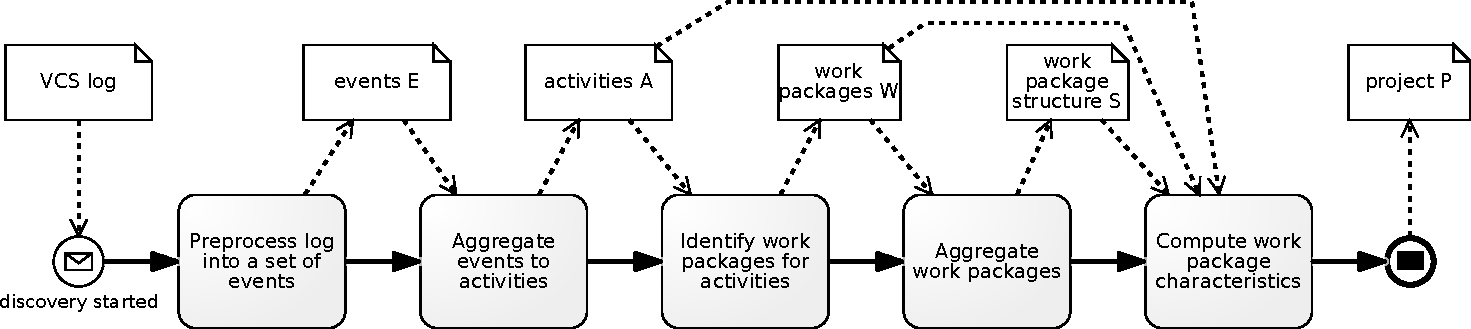
\includegraphics[width=\textwidth]{bpm2015/imgs/Project_discovery}
\caption{Project discovery technique overview as BPMN process model.}
\label{fig:project_discovery_technique}
\end{figure}
For project discovery from the \gls{vcs} commit history, we need to identify activities that are performed, associate the activities to work packages and recreate the work package structure of the project.
Our aim is to create a hierarchical model that provides an overview of the project work.
Therefore, we have to identify the start and end times of activities and of work packages before we can visualize the project work. The input to the technique is the log that is stored in the \gls{vcs}. The challenge is that the raw log only records commits on the file system level and information on activity level is missing. However, we can deduce activity information from events based on the following assumptions.

\begin{itemize}
  \item \textbf{A1: Meaningful file tree structure.} The file tree structure in a project represents its work package structure. That is, the knowledge workers organize their work in a file hierarchy that reflects the project structure.
  \item \textbf{A2: Local changes.} Activities in a work package affect only files of the work package folder, or in the corresponding sub-tree in the file tree structure.
  \item \textbf{A3: Frequent commits.} Commits to the \gls{vcs} are regularly performed, when conducting work in an activity.
\end{itemize}

Note that assumption A1 can be seen as a strong assumption on the file tree structure. Nevertheless, we argue that even if A1 is not entirely met, the aggregation of work information on the file tree hierarchy provides a valuable view on the project.
Figure~\ref{fig:project_discovery_technique} shows the different steps of the technique. We describe each of them in detail.

\subsubsection*{Step 1: Preprocessing.} The first step is to transform raw logs of version control systems (which might be grouped by commits) into a list of events as specified in Definition~\ref{def:bpm2015events}. This step is easily done by replicating the information on commit level to be contained in the events. The output is a set of events \Events.

\subsubsection*{Step 2: Aggregating events to activities.}
Given the set of events \Events that we gathered from a version control system, the next step is to identify the activities to which the events belong. Note that we do not know the activities of the project in advance, but need to infer them based on the events. Each event affects a single file in the file hierarchy.

\begin{figure}
\centering
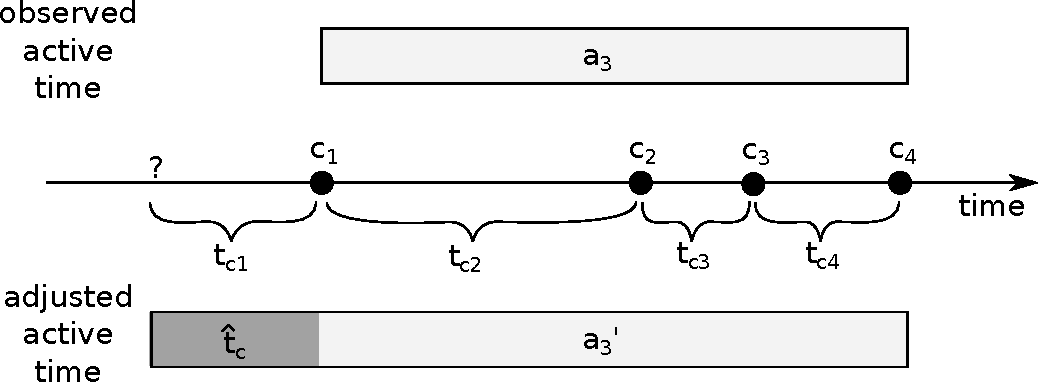
\includegraphics[width=.7\textwidth]{bpm2015/imgs/activity_adjustment}
\caption{Adjustment of activity start time \startTimeFunction. }
\label{fig:activity_adjustment}
\end{figure}

Based on assumption A2, we are interested in activities conducted in a work package, that is, we filter for the events that are contained in the given file or its children. For every file $\file$ of interest, we select the set of events affecting the file or its children as $\Events_{\file} = \lbrace \event \in \Events \mid \file = \file(\event) \vee \file \in \ancestor(\file(\event))  \rbrace$. The task is then to find the activities which emitted the set of events $\Events_{\file}$. We rely on assumption A3, which states that during an activity, we expect multiple commits. Assumption A3 allows us to conclude that if we do not observe commits for a longer period of time, there is no activity being performed in the work package.

%To derive coarse grained activities from low level events, clustering techniques~\cite{Berkhin2006ClusteringSurvey}, or abstraction functions~\cite{baier2014bridging} can be used.
%Former assume that a distance function measures the distance between events, and partitions the set of events into groups. Well-known examples are the k-means clustering~\cite{Berkhin2006ClusteringSurvey}, or hierarchical agglomerative clustering.
To this end, we adopt the abstraction technique by \citep{baier2014bridging} and allow the domain expert to formulate rules for aggregating events to activities based on boundary conditions. Assuming that people frequently commit their progress (A3), we can specify a boundary condition based on the temporal distance to previous events. For example, we can specify that a time period of seven days without a commit is a boundary condition. %But also other boundary conditions can be selected, e.g., based on resources.
As the result, we obtain the mapping from events to these activities, which we call $\eventMapping_{\file} : \Events_{\file} \rightarrow \Activities_{\file}$ in the remainder of the paper. The set of discovered activities identified for the work package based on given boundary conditions is then $\Activities_{\file} = \lbrace \activity \mid \event \in \Events_{\file}, \eventMapping_{\file}(\event) = \activity \rbrace$. We also define the inverse mapping, that is, the mapping from an activity to its events as $\eventMapping_{\file}^{-1} : \Activities_{\file} \rightarrow 2^{\Events_{\file}}$.

With the events mapped to activities, we need to find the temporal boundaries of the target activities. That is, we define the functions $\startTimeFunction$ and $\finishTimeFunction$ for each activity. The challenge here is that we do not know when an activity actually started, because the start of the activity is not recorded in the \gls{vcs}. We can only observe the time of the first commit in that activity, but commits usually mark progress of an already running activity.

To address the challenge of missing start times, we impute the missing start time by prepending the expected active time $\expectedActiveTime$ before a commit, as illustrated by Figure~\ref{fig:activity_adjustment}. This notion assumes that project participants commit their work progress after a certain amount of time. However, we cannot compute \expectedActiveTime by looking at the average commit rate in a work package, because this average is based on busy periods and idle periods. We need to factor out the idle periods in the computation of this measure.
%Therefore, we use the following formula.
%Let $\file$ be a file in the file tree that represents a work package, and let $\Events_{\file}$ be the corresponding events for all the children of $\file$. Let further $\Activities$ be the activities identified for the work package based on given boundary conditions.
We know the end time of the activities, as the last commit marks the completion of work. Therefore, each activity \activity based on given boundary conditions has the associated end time $\finishTimeFunction(\activity) = \max(\lbrace \timestamp(\event) \mid \event \in \eventMapping_{\file}^{-1}(\activity)  \rbrace)$. Further, we write the first event's timestamp of an activity as the function $\startTimeFunction'(\activity) = \min(\lbrace \timestamp(\event) \mid \event \in \eventMapping_{\file}^{-1}(\activity)  \rbrace)$.
Then, we define $\numCommits:\Activities_{\file} \rightarrow \naturalNumbers$ as the number of commits in one activity, formally $\numCommits(a)=|\lbrace \commit \mid \event \in \commit \wedge \eventMapping_{\file}(\event)=a\rbrace |$.

With this information the expected active time between commits \expectedActiveTime is given as follows.

\begin{equation}
	\expectedActiveTime = \frac{\sum_{\activity \in \Activities_{\file}} \left(\finishTimeFunction(a) - \startTimeFunction'(a)\right)}{\sum_{\activity \in \Activities_{\file}} (\numCommits(\activity)-1) }
\end{equation}

We assume that there is at least one activity spanning over at least two commits, i.e., $\exists \activity \in \Activities_{\file} \mid \numCommits(\activity) > 1 $. Translated to our boundary condition, this assumption is that there is at least one week in each work package, in which there were at least two commits made. Otherwise, we set $\expectedActiveTime$ to 0 for the current file \file due to lack of information.

Given the expected active time between commits $\expectedActiveTime$, we can finally adjust the start time of each activity. Therefore, we set the associated start time for each activity as $\startTimeFunction(\activity) = \startTimeFunction'(\activity) - \expectedActiveTime$. That is, we subtract the expected active time from the first commit's timestamp.

We apply Step 2 to all files $\file$ in the file tree to get $\Activities_\file$. For the remainder of this paper, we define the function $\fileToActivity : \Activities \rightarrow \Files$ that contains the mapping information of the discovered activities to their originating files. Finally, we set the activities \Activities in the project to be the union of the activity sets per file $\bigcup_{\file \in \Files} \Activities_\file$.

% \begin{definition}[Abstraction Function]
% Formally, we rely on an abstraction function $\abstractionFunction : 2^{\Events} \rightarrow 2^\Activities$ that maps a set of events to a set of activities.
% \end{definition}
%
% The abstraction function \abstractionFunction operates on a set of events


\subsubsection*{Steps 3 and 4: Mapping activities to work packages and aggregating.}
Once activities have been identified, we want to climb to the next abstraction layer: the work packages. Assumption A1 allows us to specify a one-to-one mapping $\kappa : \Files \rightarrow \WorkPackages$ between files in the file tree structure and work packages. More precisely, we construct the set of work packages $\WorkPackages$ isomorphic to the set of files $\Files$, such that the $\parent$ relation is preserved in the work package structure \Structure relationship. %This way, we assign the discovered activities of a selected file $\file'$ to the work package corresponding to $\file'$.

The mapping $\MappingFunction$ of activities to work packages is simply $\MappingFunction(\activity) = \kappa (\fileToActivity(\activity))$. That is, the corresponding work package of the activity that was discovered for a file.
%The aggregation of work packages is done according to the hierarchy obtained from the file tree structure.
In this way, we provide an activity based view on work packages, and we can aggregate on each level in the file system to see active periods of the corresponding hierarchy level.


\subsubsection*{Step 5: Computing work package characteristics.} In this final step, we compute measures of interest for the discovered work packages. First, we obtain the temporal boundaries of a work package by the functions $\startTimeFunction$ and $\finishTimeFunction$ of the associated activities.

Let $\MappingFunction^{-1} : \WorkPackages \rightarrow 2^{\Activities}$ be the inverse of the mapping function $\MappingFunction$ of the project.
The start and end time of a work package ($\startTimeFunction_{\WorkPackages}$ and $\finishTimeFunction_{\WorkPackages}$) are functions from work packages to timestamps. The start time is defined as $\startTimeFunction_{\WorkPackages}(\workPackage) = \min(\lbrace \startTimeFunction(\activity) \mid \activity \in \MappingFunction^{-1}(\workPackage)\rbrace )$, and the end time function of work packages $\finishTimeFunction_{\WorkPackages}$ is analogously defined using the maximum of the end times $\finishTimeFunction(\activity)$ of the activities.
We call the duration of a work package $\durationOfWorkPackage$ that is the difference between $\finishTimeFunction_{\WorkPackages}$ and $\startTimeFunction_{\WorkPackages}$.

Moreover, we are interested in the ratio of active working periods (i.e., the time spans of activities) to the total work package duration. This quantity helps to estimate the average work intensity in a work package.

\begin{definition}[Coverage]
The coverage \coverage of work packages by activities is a function $\coverage : \WorkPackages \rightarrow [0,1]$ and is defined as follows.
\begin{equation}
\coverage(\workPackage) = \frac{\sum_{\activity \in \MappingFunction^{-1}(\workPackage)}  \left(\finishTimeFunction(a) - \startTimeFunction(a)\right)}{\durationOfWorkPackage(\workPackage)}
\end{equation}

\end{definition}

With this final step, we lifted the information hidden in low level events to a high-level Gantt chart perspective, with which project managers are familiar. In the following, we compare our technique to existing process mining approaches.


% Here, we present a first approach to project mining that serves to offer a rough estimation on the work packages and their structure in a project.
% The proposed approach in this paper builds on the assumption that the file structure in the project repository is meaningful.
%
% %We acknowledge that this assumption might not be valid in all cases, but we shall demonstrate the usefulness of the approach
%
% Based on this assumption, the main task of project mining is to identify activities that are performed and map them to the work packages of the project.
%
%
%
% The approach is based on the general assumption that there is a \emph{distance} between events and we can algorithmically measure it.



% Technique: \\
%
% Algorithm (from VCS to project) \\
% \begin{verbatim}
% pseudocode of the algorithm
% \end{verbatim} 

\section{Evaluation}\label{sec:bpm2015evaluation}

In this section we evaluate our solution to the project mining problem, and show results for the example presented in Section~\ref{sec:bpm2015background}.

\subsection{Experimental setup}

%
%This section should clarify the objective of the evaluation. What do we try to study with the evaluation (which quality characteristics)? This also relates to the question whether we let the result speak for itself or if we benchmark with competing approaches. here, you should also mention that the technique was implemented as a prototype.

We evaluate our technique by a visual perspective and by comparison to possible different approaches. To this end we implemented our technique as a prototype. We used JAVA as a programming language to code the logic of our technique. For the visualization part we made use of custom SWT widgets provided by the Nebula Project\footnote{https://www.eclipse.org/nebula/}. Our program can deal with logs from Subversion (SVN) \cite{pilato2008version} and Git\cite{torvalds2010git}, but it can be extended to other version control systems by providing an implementation of the preprocessing step discussed in Section~\ref{sec:subsec:discovery_technique}.
We ran the software in an Intel\textregistered Core \texttrademark~i5-4570 CPU @ 3.20 GHz x 4 machine with 15.6 GiB of RAM and Linux kernel 3.13.0-46-generic 64-bit version.

\subsection{Input data description}

We tested our prototype with real-world log data taken from the SHAPE project. Logs were exported from the SVN and Git repositories of different projects. They come from the railway domain and describe engineering processes. Documentation stored in the repositories consists of manually produced text files, diagrams, and files coming from proprietary tools that are typically used in the domain.

We will display results for the SVN log that describes the process oriented project for SHAPE. Data span over one year, going from January 2014 to January 2015. This time window covers the phases of project definition and planning, and a part of the project execution. In the first phase, feasibility of the project was studied and budget, schedule and resources were determined. Proposal submission marked the end of this phase. The second phase started with a kickoff meeting in October 2014 and is still ongoing.

The total number of participants who actively contributed to the work packages stored in the SVN repository was 8 people in the beginning, with new resources joining the project after the kickoff date. The total number of files and directories counts up to 156 objects and 226 overall commit events. The total number of extracted change events after preprocessing (i.e. atomic changes on all the files) was 453.

The last part of the log data contains the task \defineExample, introduced in Section~\ref{sec:bpm2015problem}. For our showcase we assume that this task is contained in a work package named \emph{example}.

\subsection{Output data}

To monitor the project execution, we visualize the work progress that was done for each work package. Monitoring is performed by managers who want to have an overview on the project (which work packages are done, when and for how long, and where idleness or congestion occurs). Gantt charts offer a graphical representation for displaying schedules and jobs that were done on the various work packages \cite{wilson2003gantt} in a way that can easily be communicated to managers.

\begin{figure}
\centering
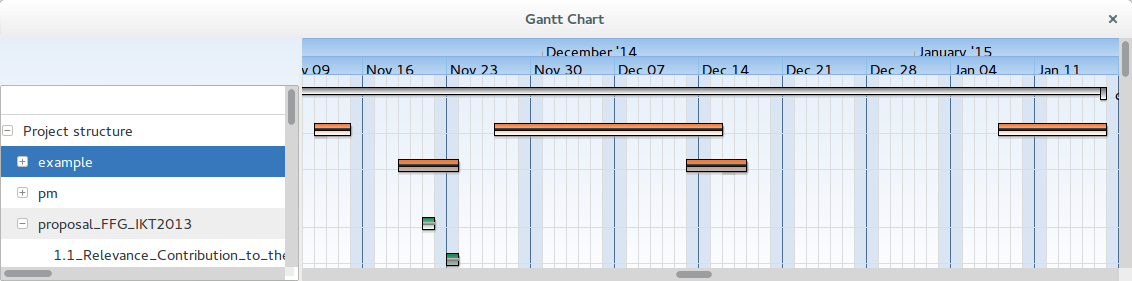
\includegraphics[width=\textwidth]{bpm2015/imgs/aggregation_and_not}
\caption{Data representation from our tool. Atomic events are drawn as dot with a minimal duration and different color per commit. }
\label{fig:example-screenshot}
\end{figure}

Figure~\ref{fig:example-screenshot} is a screenshot of how our tool presents the data. The tree structure on the left represents the \parent relation in the file tree. Events belonging to the same commit have the same color. On the top part of the chart we can see the result of merging events to activities with our aggregation method. Here we have merged the events of the example scenario on their highest abstraction level. The chart shows the three main activities and the idle times between them. %It is possible now to have an overview of the three main active periods in the work package.
On the other hand, in correspondence to expanded directories we show only their status before the aggregation. That is, every time a directory is fully expanded we apply a disaggregation into the corresponding activities. In this way, we can also show the finest granularity of work, i.e. the atomic events.

\subsection{Project Analysis}
Next, we apply our algorithm to the example case from Table~\ref{tab:bpm2015example} and check how it helps to identify work packages. The data is aggregated according to our threshold of seven days. We can observe three groups of events being temporally close to each other according to our threshold. That is, we expect the event data to be grouped into three activities.

The second step of our algorithm takes care of adjusting the starting time of the activities. Furthermore, we vertically order the events and activities in the Gantt chart according to the directory structure to show the mapping from the objects on the Gantt chart to each work package in the tree structure. The last step, computing work package characteristics is done automatically when we collapse a node on of tree.

\begin{figure}
\centering
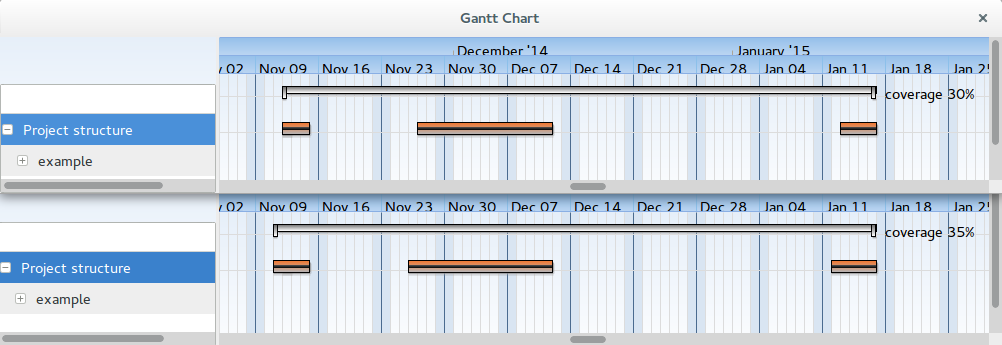
\includegraphics[width=\textwidth]{bpm2015/imgs/coverage_before_and_after}
\caption{Before and after the prepending the expected time before commit. Coverage factor increases when we adjust the starting times of the activities.}
\label{fig:example-collapsed}
\end{figure}

Figure~\ref{fig:example-collapsed} shows a comparison of the case when we do not implement the activity adjustment to the case which adjusts it. In the upper part, activity boundaries are based only on the first commit time that we see in the data. In the lower part, we observe that the start times were adjusted by approximately one day. The tool automatically adjusted the start time of the activities. As a consequence, the coverage factor increases because we expect that there was more work than what we observe by only considering the first commit time.

\subsection{Coverage tests on available open projects}

Finally, we apply our approach on different input data from open source projects. We are interested in exploring how the coverage factor varies in different existing projects. Hence, we take the work package $\workPackage$ as our controlled variable and set it to the highest level of aggregation. Then, we analyze each project of the data set and observe the dependent variable $\coverage(\workPackage)$.
Another variable of interest is the $\expectedActiveTime$ since it gives an idea of the average work speed (commit frequency) during active times.

\begin{table}
\caption{Coverage results for different open source projects}
\label{tab:experiments}
\centering
\begin{tabular}{rcccccc}
%\hline\noalign{\smallskip}
\toprule
\textbf{Log} ~&~ \textbf{Duration} ~&~ \textbf{Idle periods} ~&~ \textbf{Files} ~&~	 \textbf{Commits} ~&~	\textbf{$\expectedActiveTime$} ~&~ \textbf{$\coverage(\workPackage)$}\\
File name ~&~ Days ~&~ Number ~&~ Number ~&~ Number ~&~ Hours ~&~ \% \\ \midrule
%\hline \hline
%\noalign{\medskip}
MiningCVS &	24 & 0 & 89  &	 63 & 9 & 100 \\
%\hline

Whitehall & 1279 & 6 & 6539  &	15566 & 2 & 95 \\
%\hline

Petitions &	834 & 17 & 1562  &	914 & 13 & 59 \\
%\hline

Study &	624 & 13 & 7501  &	736 & 11 & 58 \\
%\hline

The Guardian &	1667 & 59 & 12889  &	 621 & 30 & 44 \\
%\hline

Book &	414 & 15 & 154  & 592 & 5 & 32 \\
%\hline

Papers &	 1859 & 55 & 1791  &	 649 & 20 & 30 \\
%\hline

Requirements & 771 & 22 & 505  &	231 & 17 & 21 \\
%\hline

Yelp &	206 & 6 & 24  &	54 & 20 & 20 \\
%\hline

Adobe &	1076 & 13 & 356  &	237 & 24 & 15 \\ \bottomrule
%\hline

\end{tabular}%\\ \hfill
\end{table}

%We test our tool on log data from open source projects that we find available on the web and data from SHAPE.
The data we used stems from the following projects. \emph{MiningVCS} is our tool. It consists of daily commits and was developed over 24 days.
\emph{Whitehall} is the code name for the Inside Government project, which aims to bring Government departments online in a consistent and user-friendly manner. \emph{Petitions} is a Drupal 7 code base used to build an application on "We The People", the platform to create and sign petitions of the White House.
\emph{Study} is an SVN log about Healthcare domain, taken from SHAPE.
\emph{The guardian} is the log data from the Git repository of the well-known British national daily newspaper.
\emph{Book} is the log data that describes the writing of the book Crypto 101 by Laurens Van Houtven, taken from Git.
\emph{Papers} is taken from SHAPE project for building a paper archive. %Reflects the history of collecting knowledge.
\emph{Requirements} log data is taken from the the Git repository of OpenETCS and belongs to the railway domain.
\emph{Yelp} is the main Github page of Yelp were they showcase all their projects.
\emph{Adobe} is the Adobe Github Homepage v2.0, which is a central hub for Adobe Open sources projects.

Table~\ref{tab:experiments} shows our experiments on the above-mentioned logs and the corresponding coverage factors. Projects that score a high coverage factor are characterized by continuous work. This can be further seen by looking at their average idle times $\avgIdleTime$. Let $n_c$ be the number of commits per work package. We compute the average idle time as follows.
\begin{equation}
\avgIdleTime = \frac{\durationOfWorkPackage  - n_c \cdot \expectedActiveTime }{n}
~,~ n>0
\end{equation}
where $n $ is the number of idle times in the work package. If $n=0$, then we trivially assign $\avgIdleTime = 0$, because there were no break periods over time.

Applying the formula to the above projects, we can observe how projects with a higher coverage factor have actually low values of $\avgIdleTime$. For instance, \emph{Whitehall} scores a $\avgIdleTime$ of 11 days, whereas \emph{Adobe} scores a $\avgIdleTime$ of 36 days.
This supports the usage of the coverage factor $\coverage$ as an indicator for work package time utilization. 

\section{Discussion}
\label{sec:bpm2015discuss}

In this section we compare our method to other alternatives for mining data out of logs and interpret our results.

Well known tools that are used in academia and practice include ProM\cite{van2005prom} and Disco\footnote{http://fluxicon.com/disco/}. Both tools require input data to be in the XES~\cite{Verbeek2011} format. Thus, we convert our data from the $\defineExample$ case into XES. To show events per objects of the project structure, we choose the file path as the \emph{caseId}. To flatten the logs we extract all the file paths and build a mapping from each file to the set of changes done to it.

Figure~\ref{fig:dottedchart} depicts the results of the Dotted chart plugin of ProM applied to our log data. Also here, we observe different changes of each file of the repository. While the files and their corresponding events are shown, the plugin does not allow to rearrange the data in order to understand the file structure, nor does it allow to perform any kind of aggregation or connection between data, to observe them from a higher level perspective.

Figure~\ref{fig:discochart} shows the results from mining our log data with the Disco tool. Here we can see a plot that displays the events that happen over time. The plot has some peeks in correspondence to active times of the \emph{example} work package. They can be grouped in three clusters: an initial cluster with a few amount work, an intermediate cluster with the most significant part of the work, and a final cluster that again is not very active. In this way, clusters can be associated to activities. As a drawback, when the number of work packages and activities increase, the number of peeks grows and generate identifying clusters of activities by look at active (or idle) times becomes unworkable.

\begin{figure}
\centering
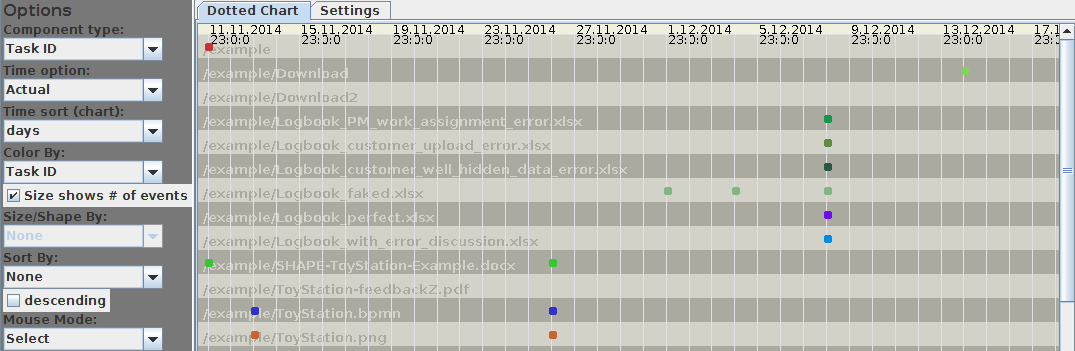
\includegraphics[width=\textwidth]{bpm2015/imgs/dotted_chart_ordered_by_taskID_cut}
\caption{Dotted chart from ProM}
\label{fig:dottedchart}
\end{figure}


\begin{figure}
\centering
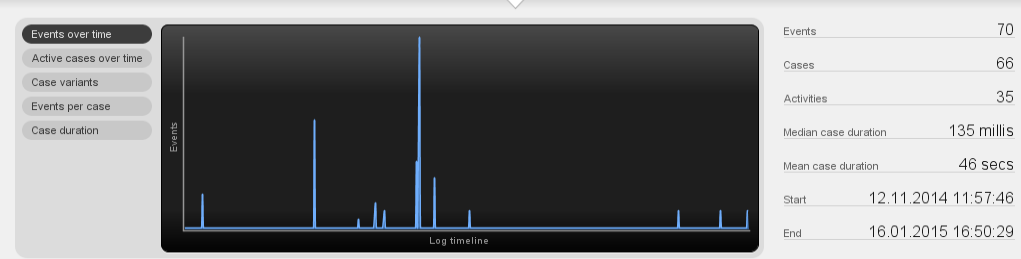
\includegraphics[width=\textwidth]{bpm2015/imgs/disco_screenshot_chart}
\caption{Chart from Disco plotting the events over time.}
\label{fig:discochart}
\end{figure}

Our approach to mining the work progress of project-oriented business processes complements these techniques with metrics and a corresponding visualization that is informative to managers.

\section{Summary}
\label{sec:bpm2015outro}

In this chapter we
%identified a new a class of business processes that are executed according to planned data, resources and time constraints, to achieve predefined goals. We
addressed the problem of mining and visualizing project-oriented business processes in a way that is informative to managers. We define an approach that takes VCS logs as input to generate Gantt charts.
%provided a formal description to capture the project-oriented class of business processes. We presented an approach to mine them as Gantt charts from VCS logs.
Our algorithm works under the assumptions that repositories reflect the hierarchical structure of the project, each work package is contained in a corresponding directory and project members commit their work regularly during active working times.
The approach was implemented as a prototype and evaluated based on real-world data from open source projects.
%We implemented our method as a prototype tool that can visualize the project hierarchy along with events and activities for each level, by aggregation or disaggregation.
%Compared to classical process mining, our method offers a better overview on project structure and on the characteristics of work packages.
%Tests on real-world data, both from open source projects and from SHAPE, show how our metric on work packages can help to better understand work how efficiently they utilize their time.

In future work, we aim to extract further details of the VCS logs in order to calculate metrics that approximate the work effort. %\todo{Point 4 on the reviews: Add a discussion on how the project mining approach can is affected by different projects characteristics: number of commits, number of files, number of activities, duration of the project, number of participants, etc. } 
We plan to investigate on how the project mining approach is affected by project characteristics. Furthermore, we want to utilize statistical methods to better estimate the boundaries of the activities and work packages. Finally, we have already incorporated feedback from managers and plan to extend these to full user studies.

%from a more granular perspective, looking also into the parts of a file that were affected by a change. We also want to investigate ways that help us to better understand the boundaries of activities and work packages. We take into account using natural language processing techniques on the comments associated to commits and analyze their semantics. Furthermore, we want to consider clustering techniques in order to relax our assumptions on the directory structure.
